\subsection{System Requirements}

\subsubsection{JDK}
In case you don't have any version of Java Development Kit you should download its latest version from:
\\
\href{url}{http://www.oracle.com/technetwork/java/javase/downloads/jdk8-downloads-2133151.html}

\subsubsection{Glassfish Web Server}
Being Travlendar+ a web application, it is essential to have a web server installed, here we provide information about the installation and deployment on Glassfish 4.1.1. You can download it from
\\
\href{url}{https://javaee.github.io/glassfish/download}
\\or alternatively, you can follow the quick installation instructions for Windows, which includes a Glassfish installation.

\subsubsection{DBMS}
For simplicity, we decided to use the basic DBMS provided by glassfish, Apache Derby RDBMS, thus you do not need anything else if you have installed Glassfish Server.

\subsubsection{Browser}
For the development and testing we always used Google Chrome as browser, we recommend installing the latest version of Chrome and we do not guarantee the absence of bugs and poor performances on other Browsers, even if they would probably work just as fine.

\subsection{Quick Installation for Windows}
The quick installation consists in downloading Glassfish 4.1.1 with the script to install Travlendar and the war file already in it.
\begin{itemize}
\item Download the JDK if you don't have it already from\\ \href{url}{http://www.oracle.com/technetwork/java/javase/downloads/jdk8-downloads-2133151.html}, usually it is stored in C:\textbackslash Program Files\textbackslash Java, put it there or wherever you prefer, keep in mind or save the path where you put it.
\item Download the zip at: \href{url}{https://}, unzip the folder and put the folder glassfish-4.1.1 it contains in C:\textbackslash Program Files.
\item Open the glassfish-4.1.1 folder and double click on installtravlendar file.
\item Click yes to the popup that asks if you want to run it as administrator.
\item Write down in the Command Prompt the JDK path when asked for it, for example write: C:\textbackslash Program Files\textbackslash Java\textbackslash jdk1.8.0_121
\item Press enter.
\item If everything went fine the default browser should have been launched and you should see the login page of the app, signup and enjoy the app.
\end{itemize}




\subsection{Manual installation - Environment Setup}
\subsubsection{Starting up Glassfish Server}
\begin{itemize}
\item On Windows, open command prompt as administrator (right click on cmd.exe and click Run as administrator), on Linux or MacOS open Terminal.
\item browse to Glassfish installation path and open bin folder, usual installation path on Windows: \textit{C:\textbackslash Program Files\textbackslash glassfish-4.1.1\textbackslash bin}, execute command \textit{cd C:\textbackslash Program Files\textbackslash glassfish-4.1.1\textbackslash bin}
\item execute command \textit{asadmin start-domain}
\end{itemize}

\begin{figure}[H]
\begin{center}
		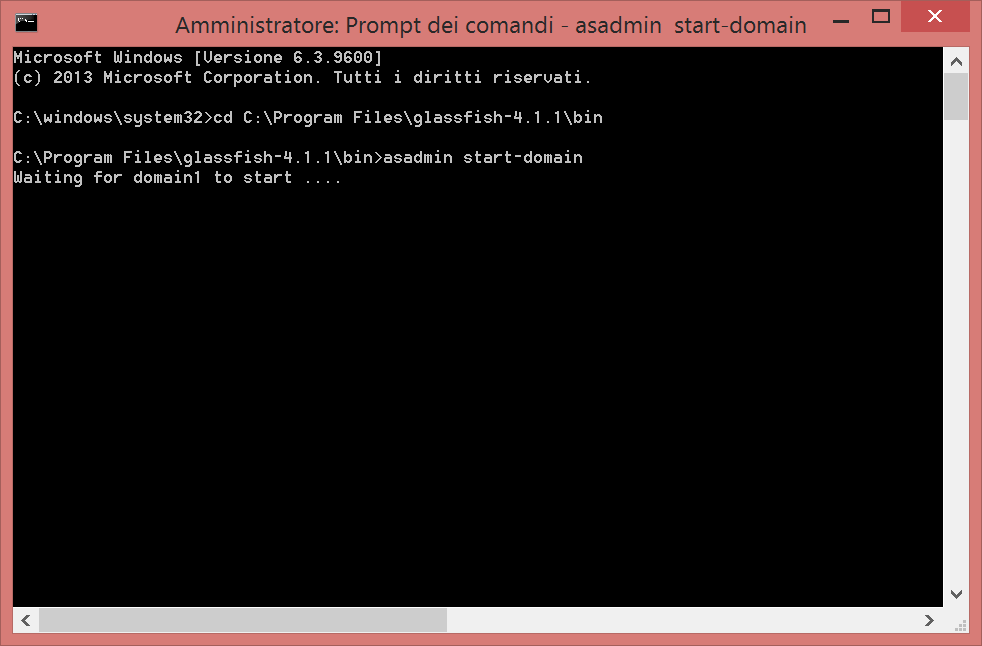
\includegraphics[width=1.1\textwidth]{images/asadminstart}
		\caption{Commands to execute in order to start Glassfish Server}
		\label{asadminstart}
\end{center}
\end{figure}

After the server has started you will be able to access the Admin Console at  \\
\href{url}{https://localhost:4848} and the web server at \\
\href{url}{https://localhost:8080} 
\\(If you need to stop Glassfish server just execute command \textit{asadmin stop-domain}

\subsubsection{Setting up JDK path}
Sometimes an error is displayed if Glassfish does not find the JDK automatically, you can execute the command \\ \textit{asadmin set "server.java-config.java-home=C:\textbackslash Program Files\textbackslash Java\textbackslash jdk1.8.0_121"} \\
Just substitute \textit{C:\textbackslash Program Files\textbackslash Java\textbackslash jdk1.8.0_121} with your path to the JDK you previously downloaded.

\subsubsection{Database configuration}
In order to make it simpler to create the database you can download the already configured Derby database from \\
\href{url}{https://linkdropbox}
\\Unzip it and put it in the folder: \textit{.\textbackslash glassfish\textbackslash databases}\\ in the glassfish installation path (on Windows usually \\
\textit{cd C:\textbackslash Program Files\textbackslash glassfish-4.1.1}
\begin{figure}[H]
\begin{center}
		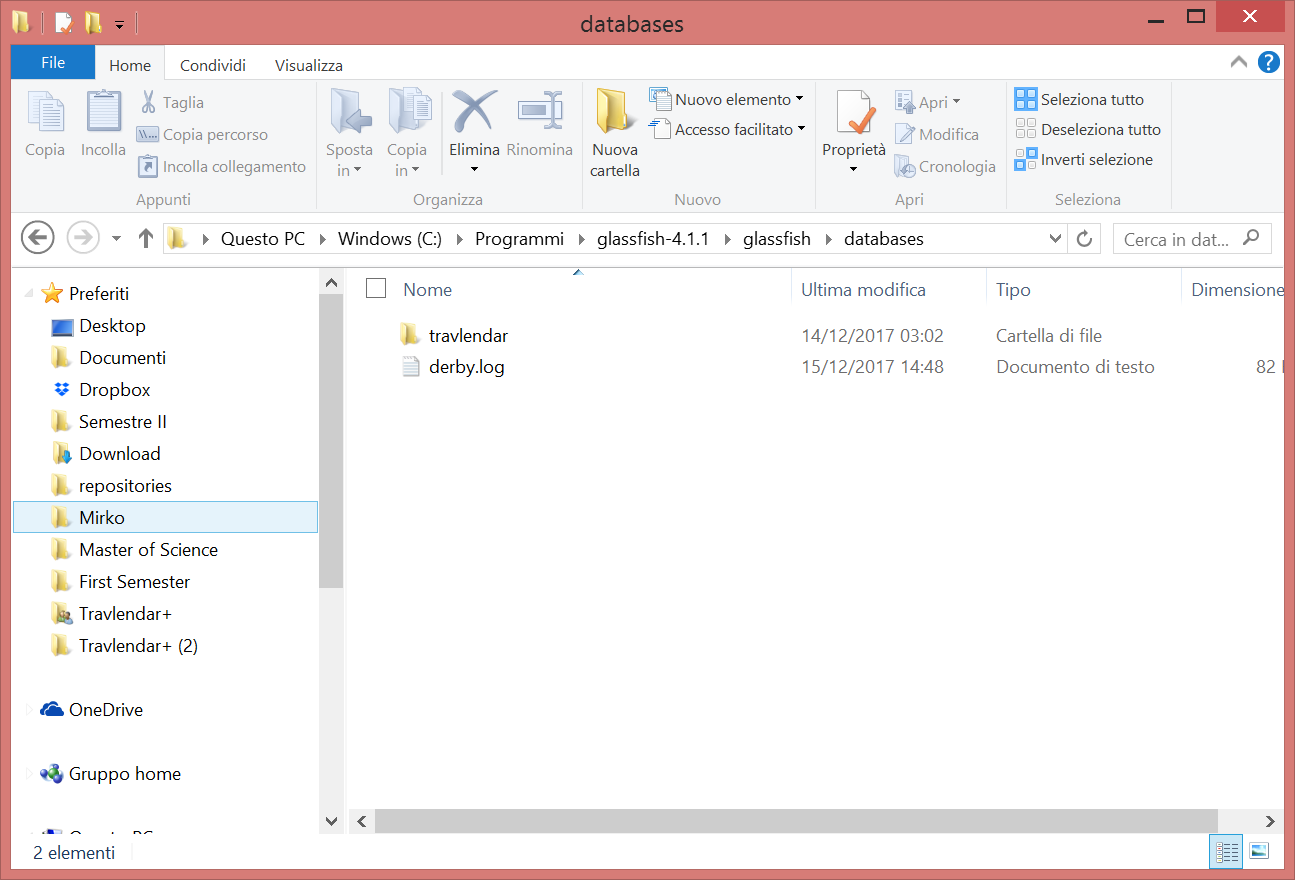
\includegraphics[width=1.1\textwidth]{images/databaselocation}
		\caption{Location in which the database should be stored}
		\label{asadminstart}
\end{center}
\end{figure}


\subsubsection{Starting Apache Derby DBMS}
Execute command \\
\textit{asadmin start-database} \\ in order to start the database. 
\begin{figure}[H]
\begin{center}
		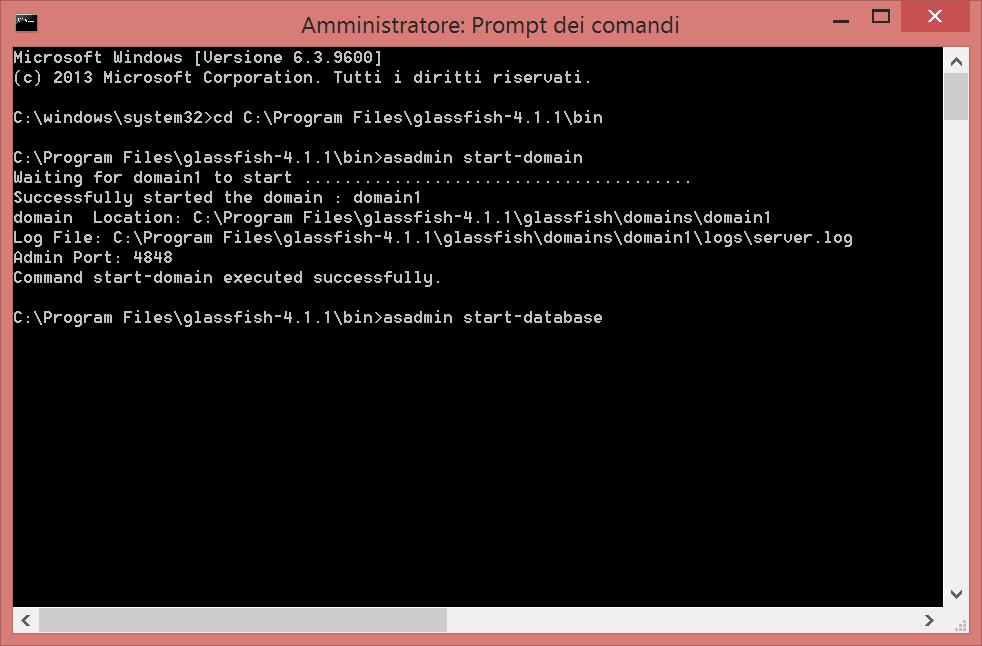
\includegraphics[width=1.1\textwidth]{images/asadmindatabase}
		\caption{Commands to execute in order to start Apache Derby DBMS}
		
\end{center}
\end{figure}
Be sure the port is the default one (1527). \\
If at any moment you want to stop the database just execute command \\
\textit{asadmin stop-database}


\subsection{Application Deployment}
After having configured and set up the environment, download the \texttt{.war} file \texttt{Travlendar.war} at \\
link release in github.
\\You can now follow one of these ways in order to deploy the Application on Glassfish.

\subsubsection{Manual deployment from Admin Console}
After the server has started you will be able to access the Admin Console at  \\
\href{url}{https://localhost:4848}
\\Click on \texttt{Applications} tab on the left. Then click \texttt{Deploy...} button.

\begin{figure}[H]
\begin{center}
		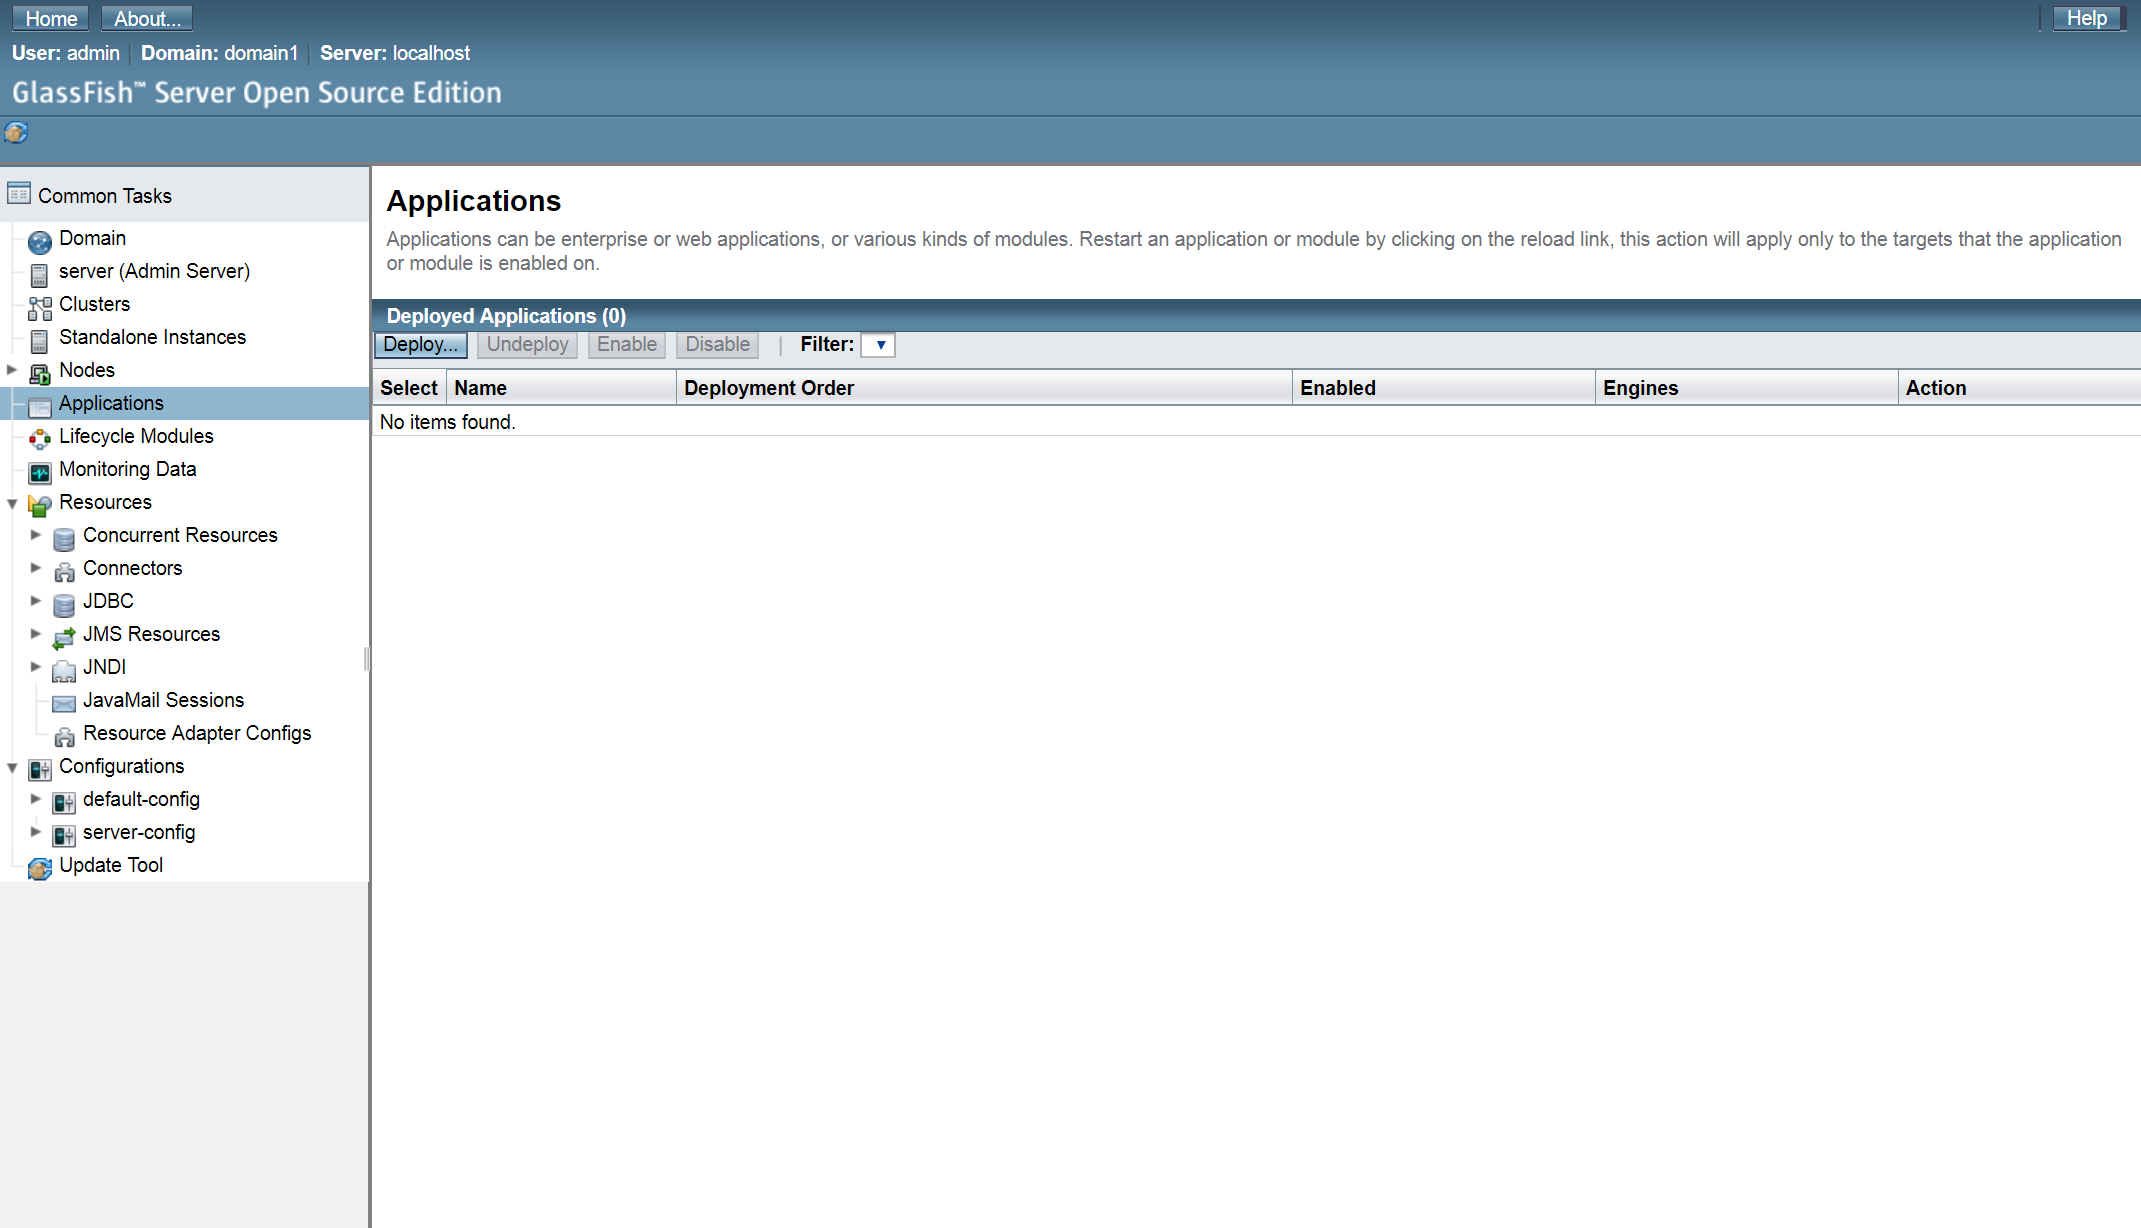
\includegraphics[width=1.1\textwidth]{images/glassfishconsole}
		\caption{Glassfish admin console}
		
\end{center}
\end{figure}

Click on \texttt{Choose file} and select the \texttt{Travlendar.war} release file previously downloaded, then click ok.

\begin{figure}[H]
\begin{center}
		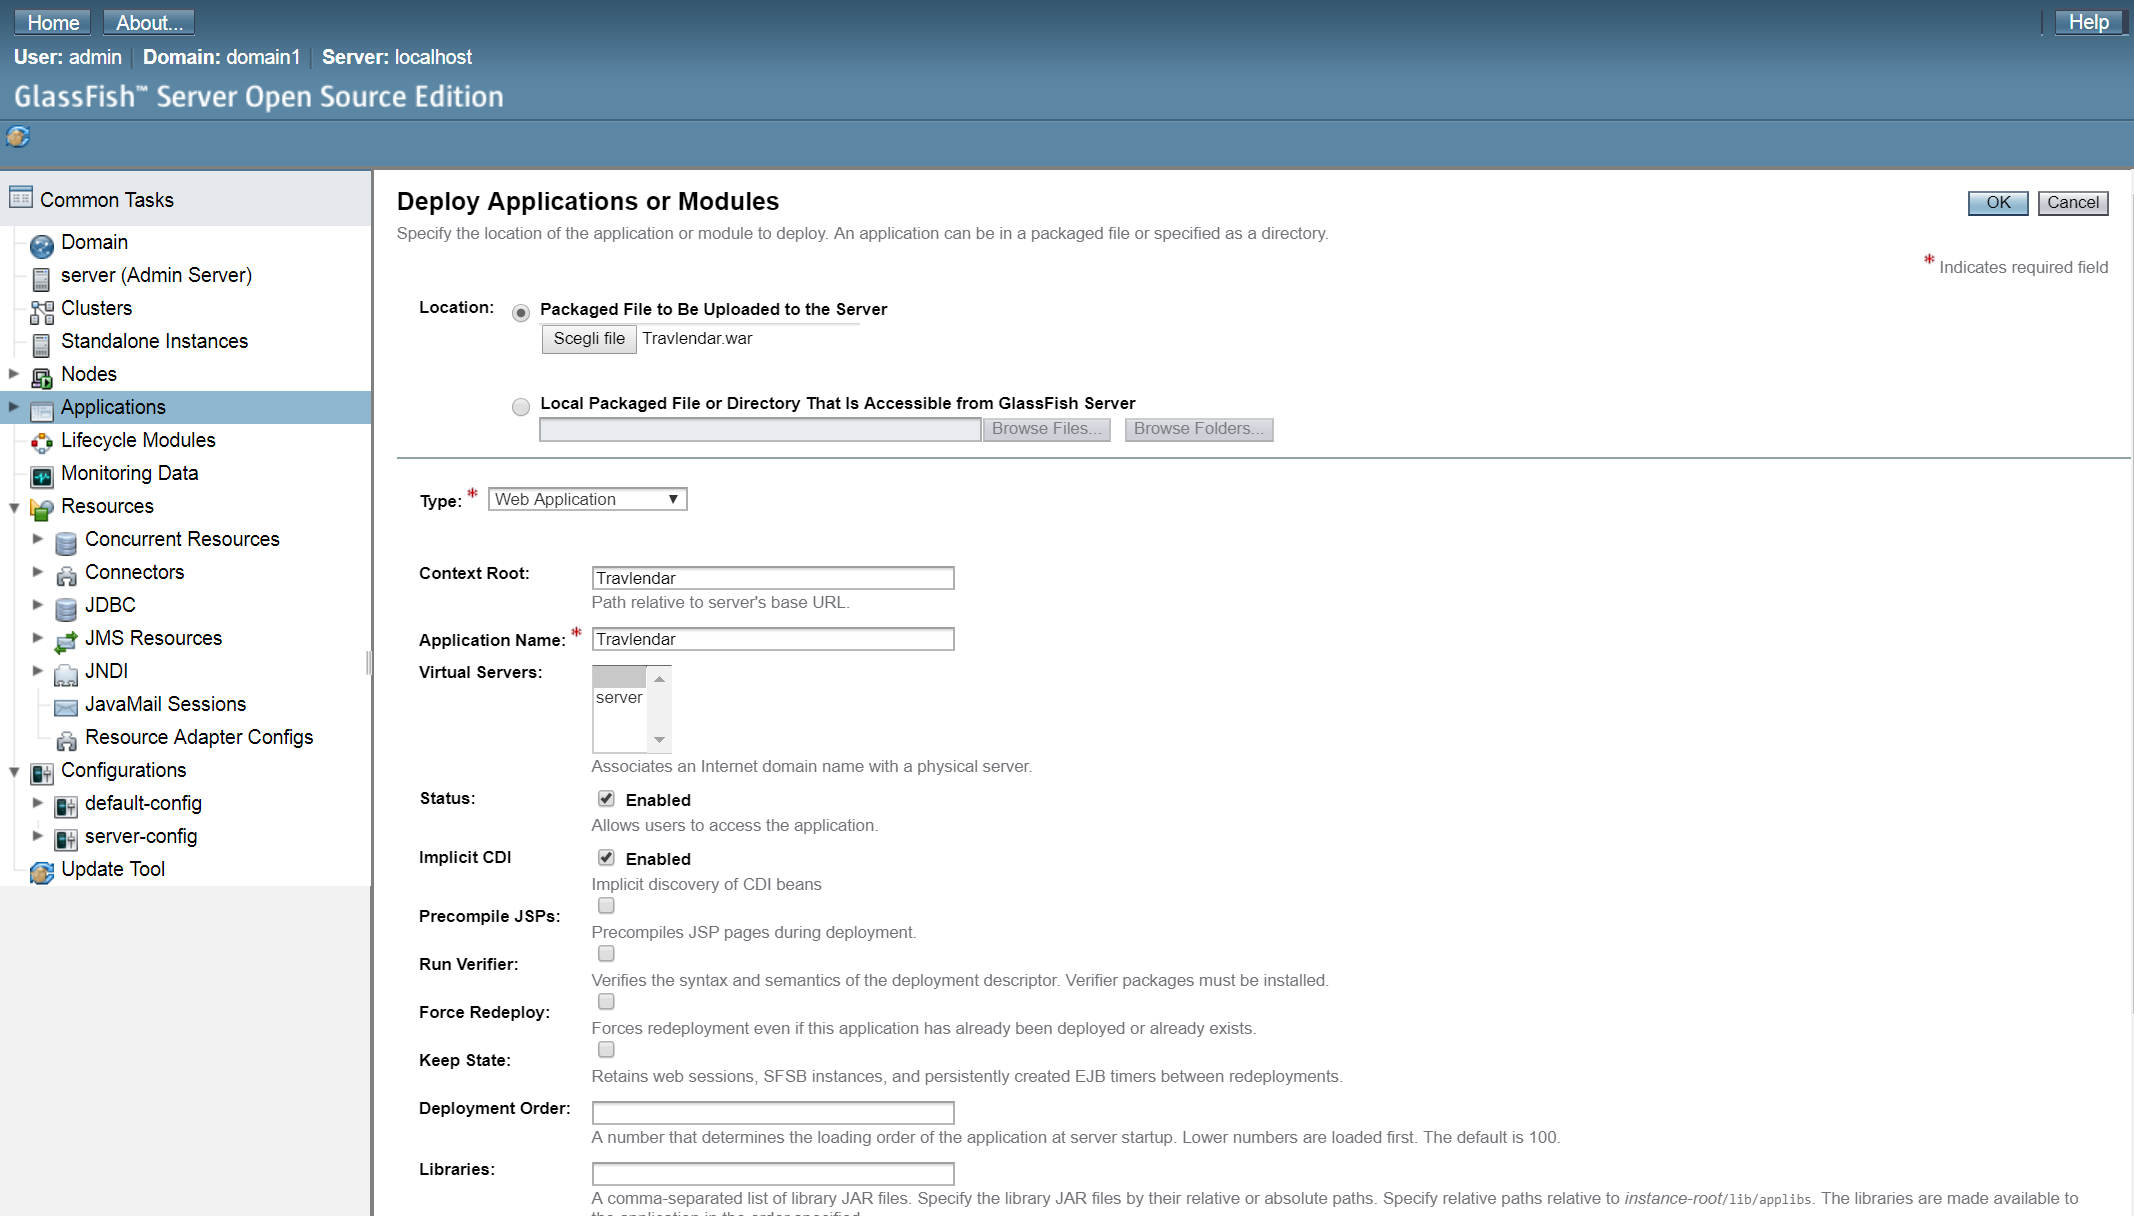
\includegraphics[width=1.1\textwidth]{images/glassfishdeploy2}
		\caption{Glassfish admin console}
		
\end{center}
\end{figure}

If everuthing went fine you should see something similar to this.

\begin{figure}[H]
\begin{center}
		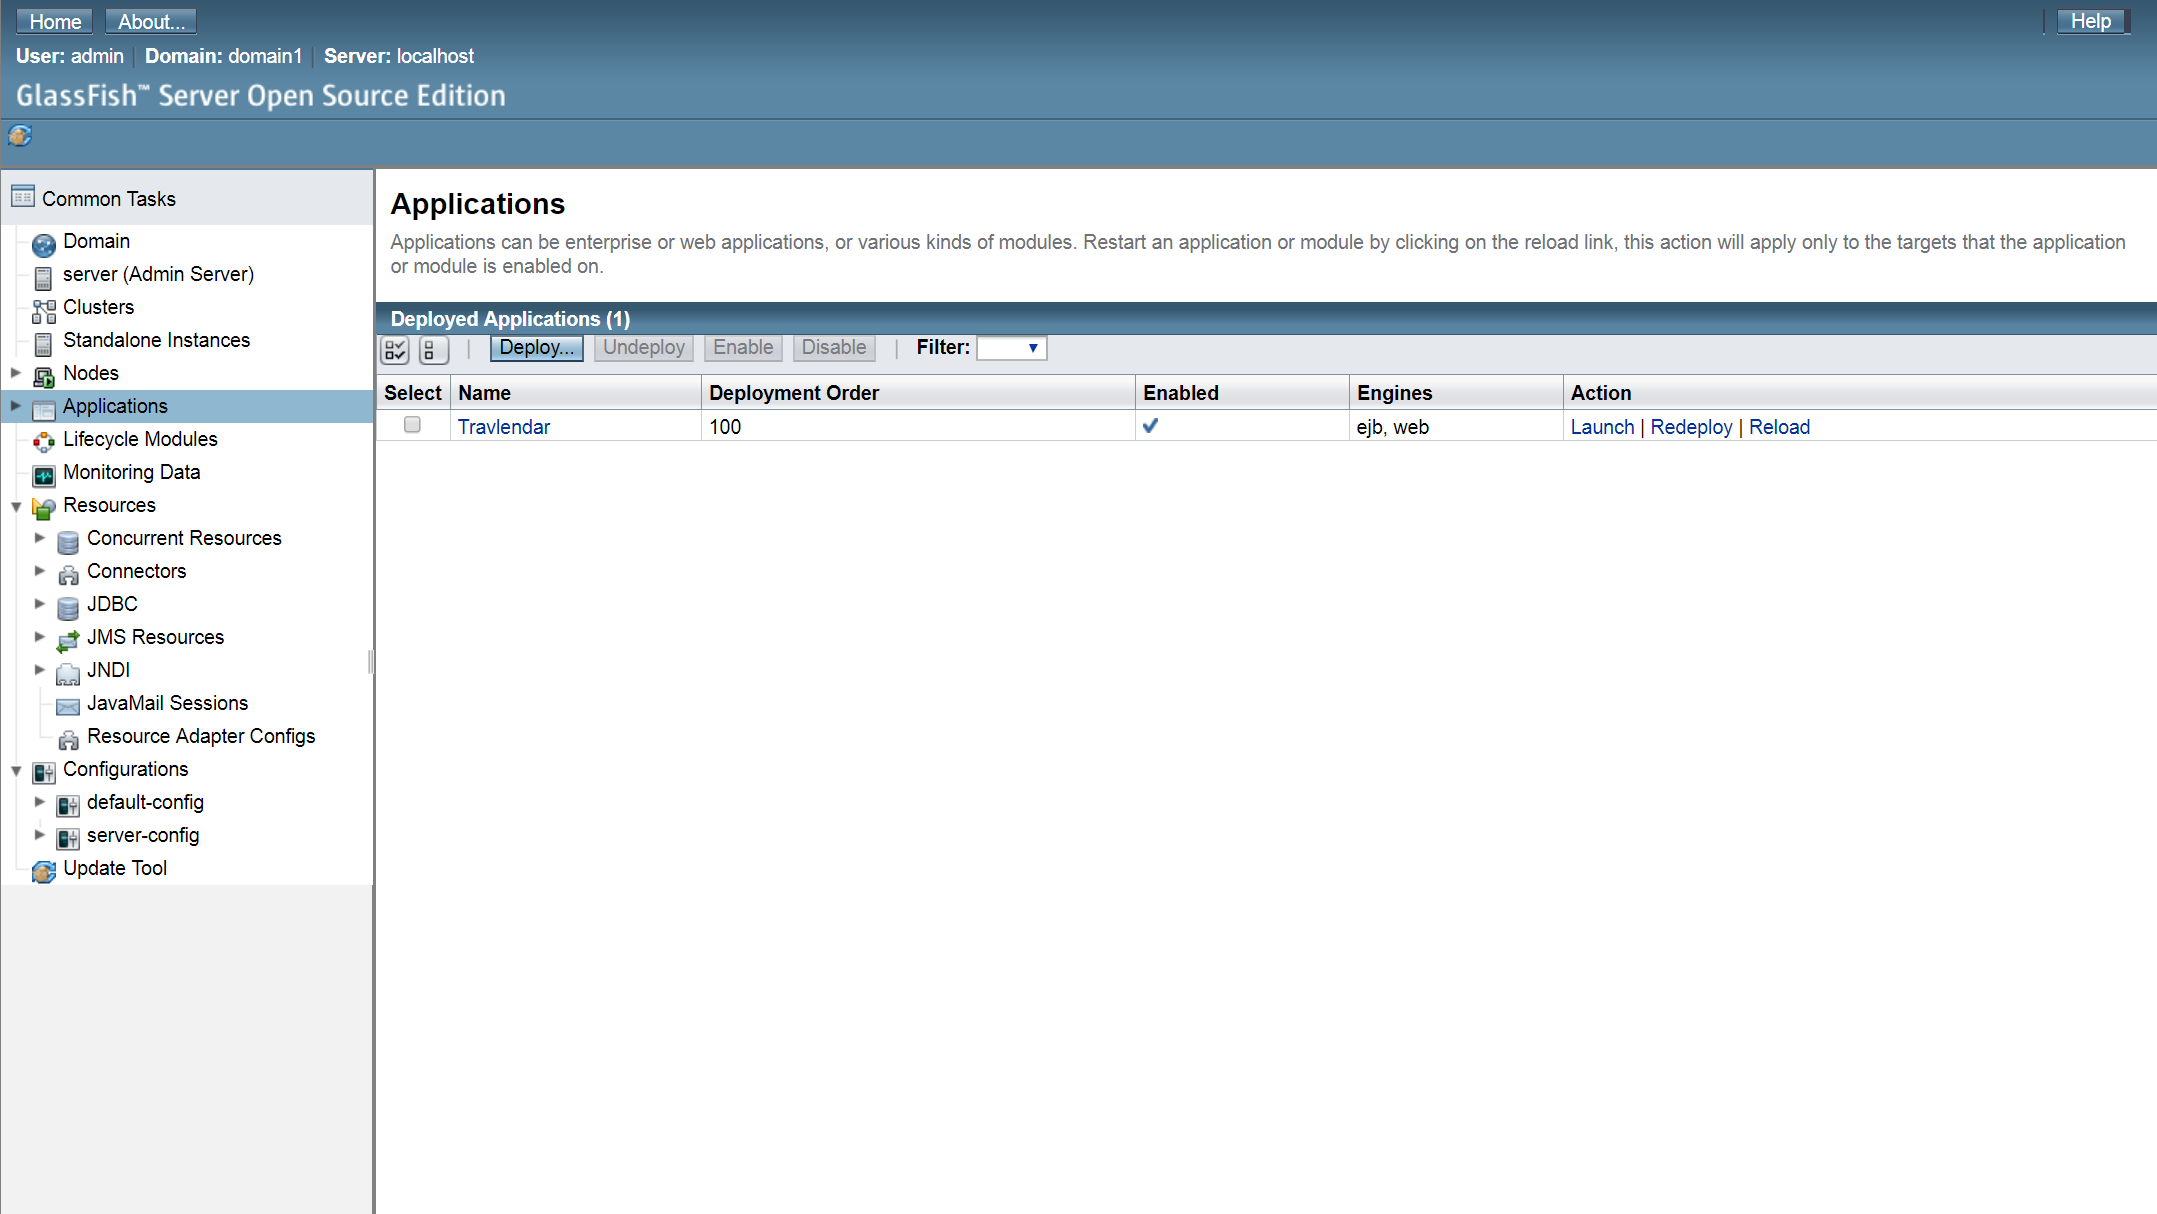
\includegraphics[width=1.1\textwidth]{images/glassfishdeploy}
		\caption{Glassfish admin console}
	
\end{center}
\end{figure}
Just click on \texttt{Launch} to start the application.
\\You can access the application opening the URL: \\
\href{url}{https://localhost:8080/Travlendar}


\subsubsection{Manual deployment from Command Line}
Supposing you already started the server and the database, and you are in the bin folder in the Glassfish installation path, just execute \\ \textit{asadmin deploy C: \textbackslash Users\textbackslash Mirko \textbackslash Desktop\textbackslash Travlendar.war}\\
substituting \textit{C: \textbackslash Users\textbackslash Mirko \textbackslash Desktop\textbackslash} with your path to \texttt{Travlendar.war} release file.

\begin{figure}[H]
\begin{center}
		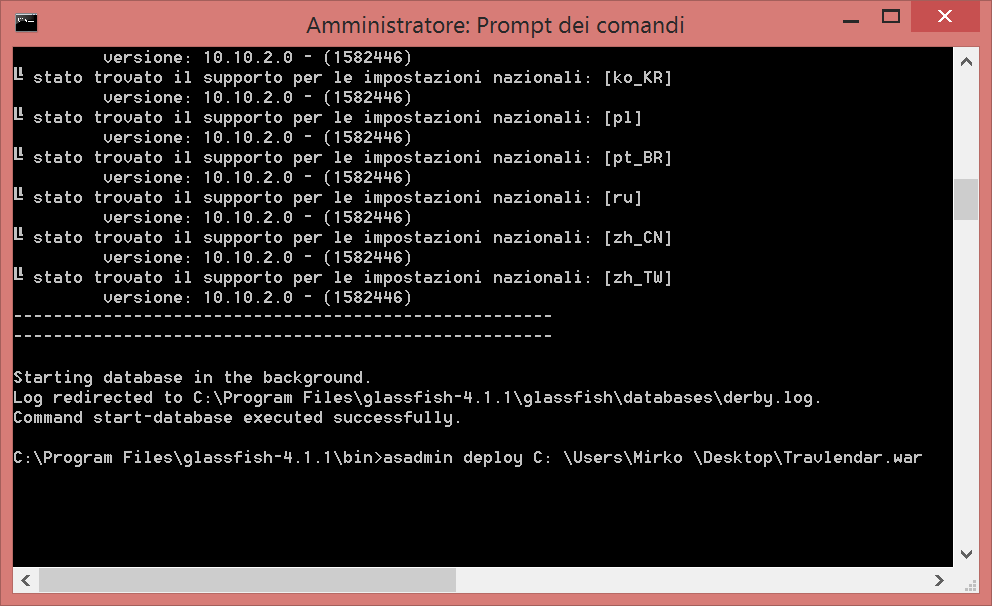
\includegraphics[width=1.1\textwidth]{images/asadmindeploy}
		\caption{Commands to execute in order to Deploy the application on Glassfish Server}
		
\end{center}
\end{figure}

You can now access the application by executing \\
\textit{start http://localhost:8080/Travlendar/} on Windows, \textit{open http://localhost:8080/Travlendar/} on MacOS X, or \textit{xdg-open http://localhost:8080/Travlendar/} on Linux, or simply open the browser and type \textit{localhost:8080/Travlendar} in the URL bar and press Enter.

\subsubsection{Autodeployment}
Just put the \texttt{Travlendar.war} file in \textit{<GlassFish-Installation-Path>/domains/domain1/autodeploy} and restart the server.

\subsection{Running the app}
Once the deployment is finished you can access the Application at \textit{localhost:8080/Travlendar}
on a browser in your local machine, at \textit{192.168.1.3:8080/Travlendar} on a device connected to the same LAN (just replace \textit{192.168.1.3} with the private IP address of the machine the server is running on. 
\\You can even access the application from a remote device, you just need to open the port 8080 of the router of your LAN by creating a virtual server and NATting the external access onto the private IP address of the machine your server is running on (private IP should be configured as static). Then you can access from wherever you want just by going to \textit{xx.xx.xx.xx:8080/Travlendar}, replace xx.xx.xx.xx with the public IP address of your router.

\begin{figure} 
\begin{center}

\makebox[\textwidth]{%
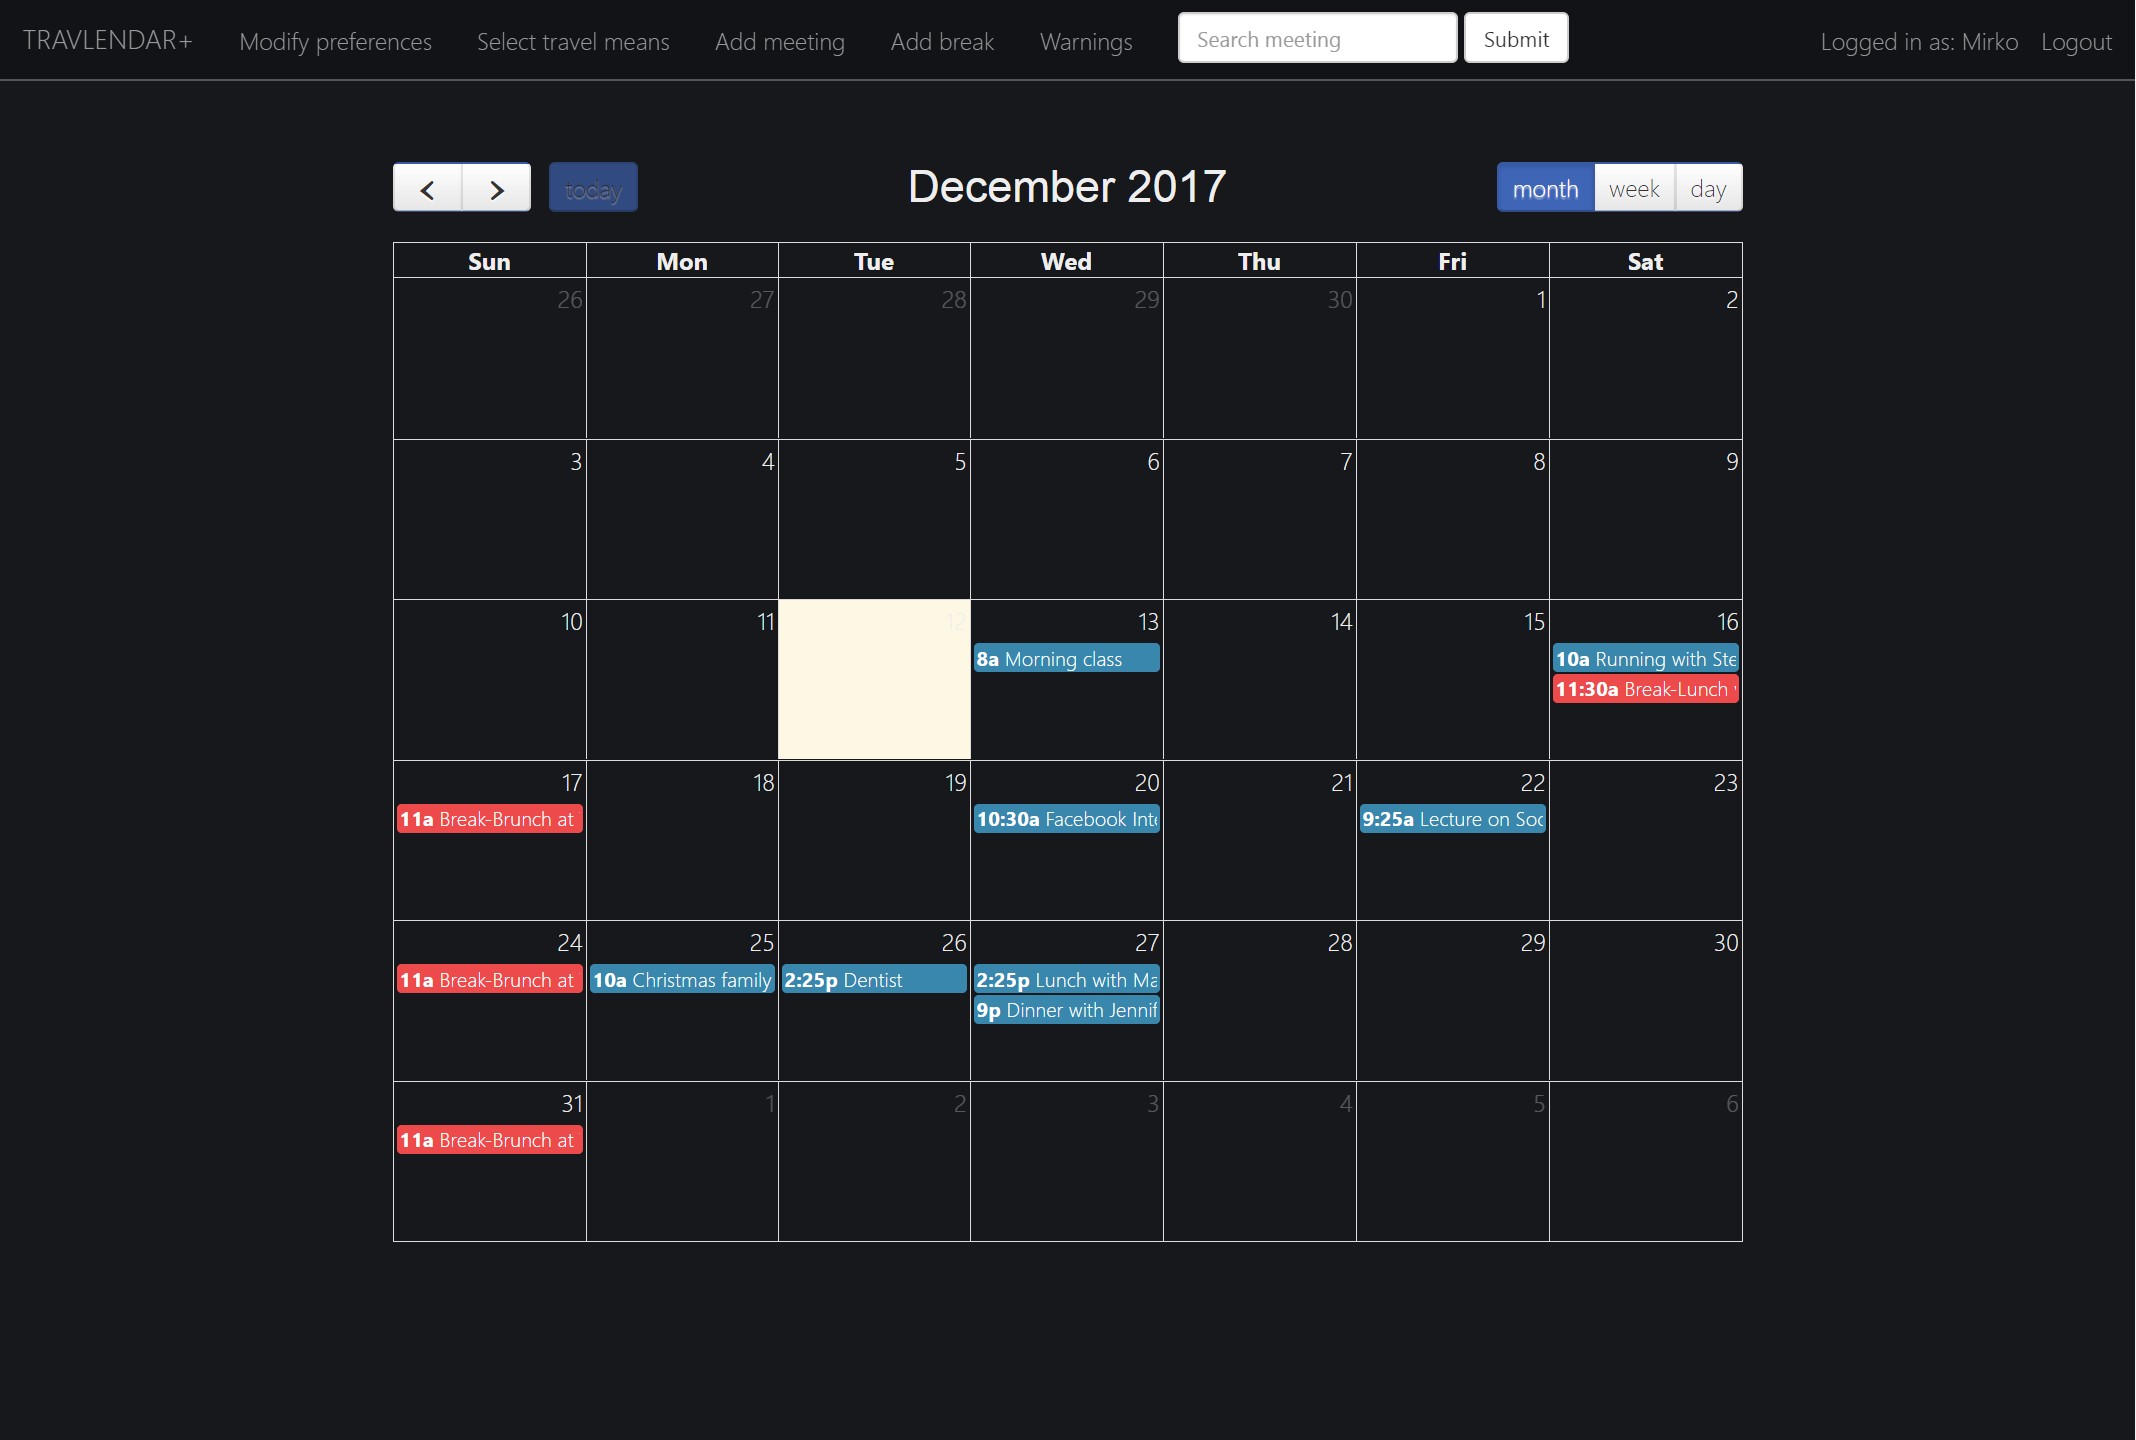
\includegraphics[width=1.5\linewidth]{images/homepage} 
}
\caption{Travlendar Homepage} 
\label{fig:travlendarhomepage} 


\end{center}
\end{figure} 

\clearpage
\subsection{Possible issues and solutions}
If you encounter any problem in the deployment regarding a database connectivity problem you could download Netbeans IDE (which includes Glassfish and Derby installation) and replace the Environment setup steps by creating a database with databasename = travlendar, name = mirko, password = mirko.
Start glassfish server from there and then pass to the deployment phase as explained in these instructions.
\\If also this does not let you deploy the app as last chance you could clone the travlendar repository, import it as a project in netbeans build and clean the project, and run it.
